\chapter{PRIME Data Headend Server}
\section{Introducción}
PRIME Data Headend Server, en adelante <<PRIME DHE>>, es un producto software capaz de sustituir un concentrador de datos tradicional en una red PRIME. <<PRIME DHE>> implementa uno o varios concentradores virtuales en un equipo servidor completamente deslocalizado de la red que administra. En conjunción con el router <<Regesta PLC 3G>> (de la compañía <<Teldat>>) como nodo base de la red, el tandem creado está habilitado para operar completamente una red PRIME. Así, se hace innecesario la instalación física de concentradores de datos, ahorrando una parte importante en costes de mantenimiento e instalación.

Para entender como trabaja <<PRIME DHE>>  primero hay que conocer la estructura de una red <<PRIME>>. La figura \ref{fig:EstructuraPRIME} representa una topología típica de una red PRIME. Los elementos que actúan en ella son los siguientes:
\begin{description}
	\item[STG] El Sistema de Telegestión es el punto de entrada del usuario operador de la red. Este se encarga de pedir periódicamente a los concentradores los informes con las medidas de consumo, y solicitar la ejecución de órdenes. Todo ello a través de servicios web.
	\item[Router] El router es el enlace de comunicaciones entre el concentrador y el STG.
	\item[Concentrador] El concentrador por su parte está constantemente preguntando a los contadores sus medidas y ejecuta las órdenes e informes que le solicite el STG. Para ello, típicamente, disponen de dos interfaces de red: una para recibir y enviar al STG (a través del router); y otra para la comunicación PLC con los contadores (a través del nodo base).
	\item[Nodo Base] El nodo base es el enlace de comunicaciones entre los contadores y el concentrador a través de la línea eléctrica.
	\item[Contadores] Los contadores son el fin último de las <<Smart Grids>>, llevan la cuenta de la energía consumida y vertida en la red eléctrica, controlan la potencia máxima de salida hacia el consumidor, etc...
\end{description}

\begin{figure}[htbp]
	\centering
	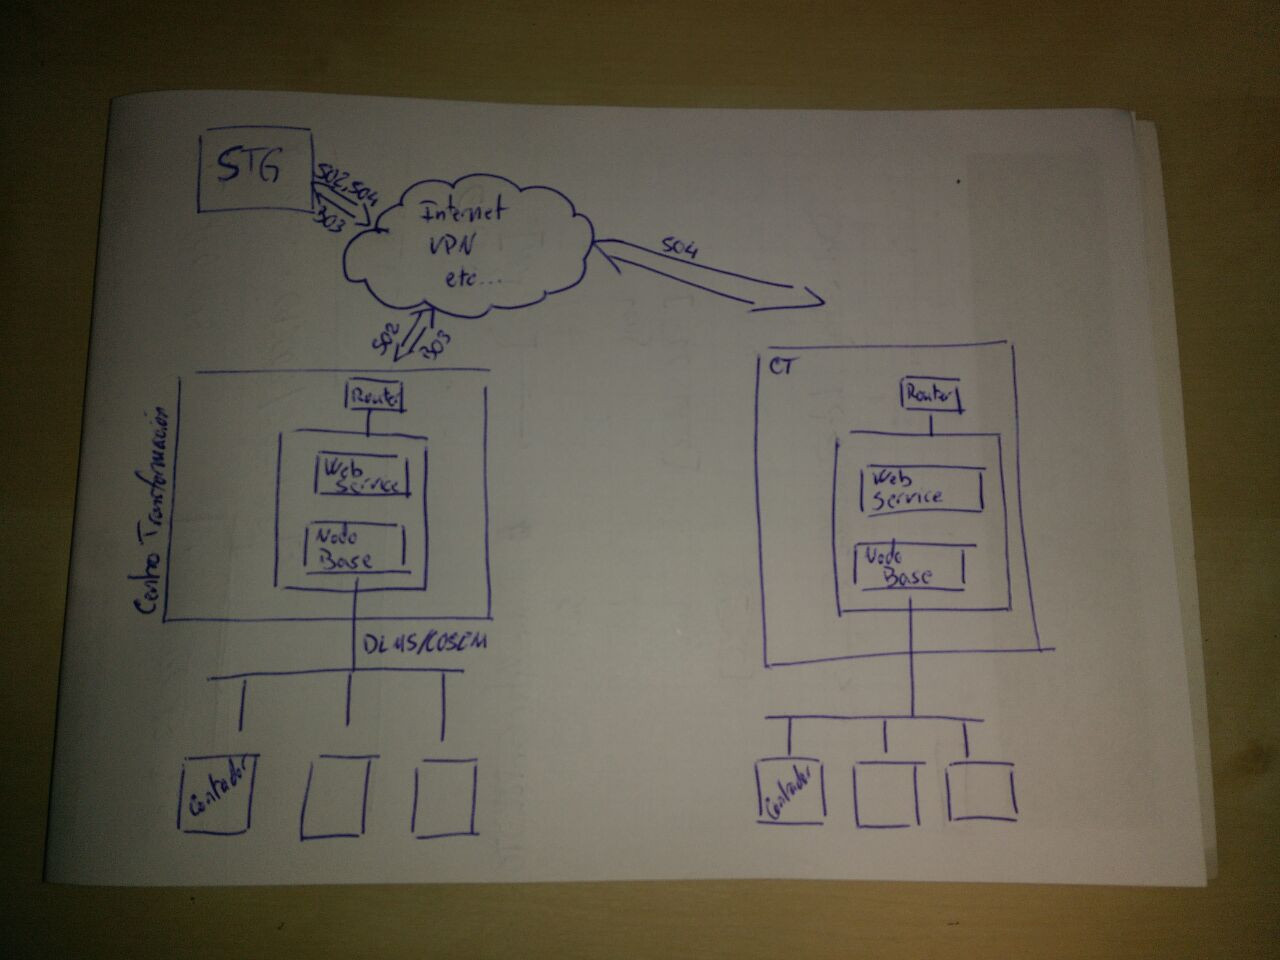
\includegraphics[width=\textwidth]{Img/boceto_estructura_prime.jpg}
	\caption{Topología de red PRIME}
	\label{fig:EstructuraPRIME}
\end{figure}

A grandes rasgos su funcionamiento sería el siguiente: el STG se comunica con el concentrador para solicitarle informes de medidas o la ejecución de alguna orden a través de los <<Web Services>>. El concentrador acepta las órdenes del STG, y las ejecuta comunicándose a su vez con los contadores a través del <<nodo base>> y enviando de nuevo la respuesta al STG. El concentrador también puede enviar informes de forma automática antes incluso de que el STG se los requiera.

En cualquier caso son bastantes dispositivos complejos los que entran en funcionamiento, con los costes de mantenimiento e instalación que conllevan. En este punto es dónde la propuesta de red de <<PRIME DHE>> muestra su primera ventaja. En la figura \ref{fig:EstructuraPrimeDHE} se observa la topología de red propuesta. En <<PRIME DHE>> se elimina el concentrador tradicional, y en su lugar se instala un router un tanto especial, este router contiene un nodo base PRIME al que podemos acceder para las comunicaciones con los contadores. Así, toda la lógica del concentrador es sustituida por <<PRIME DHE>>. Al ser un producto software, se pueden controlar varios nodos base con una sola instancia de <<PRIME DHE>>, con lo que se reducen los costes de operación, se homogeneiniza el funcionamiento y se gana en fiabilidad.

\begin{figure}[htbp]
	\centering
	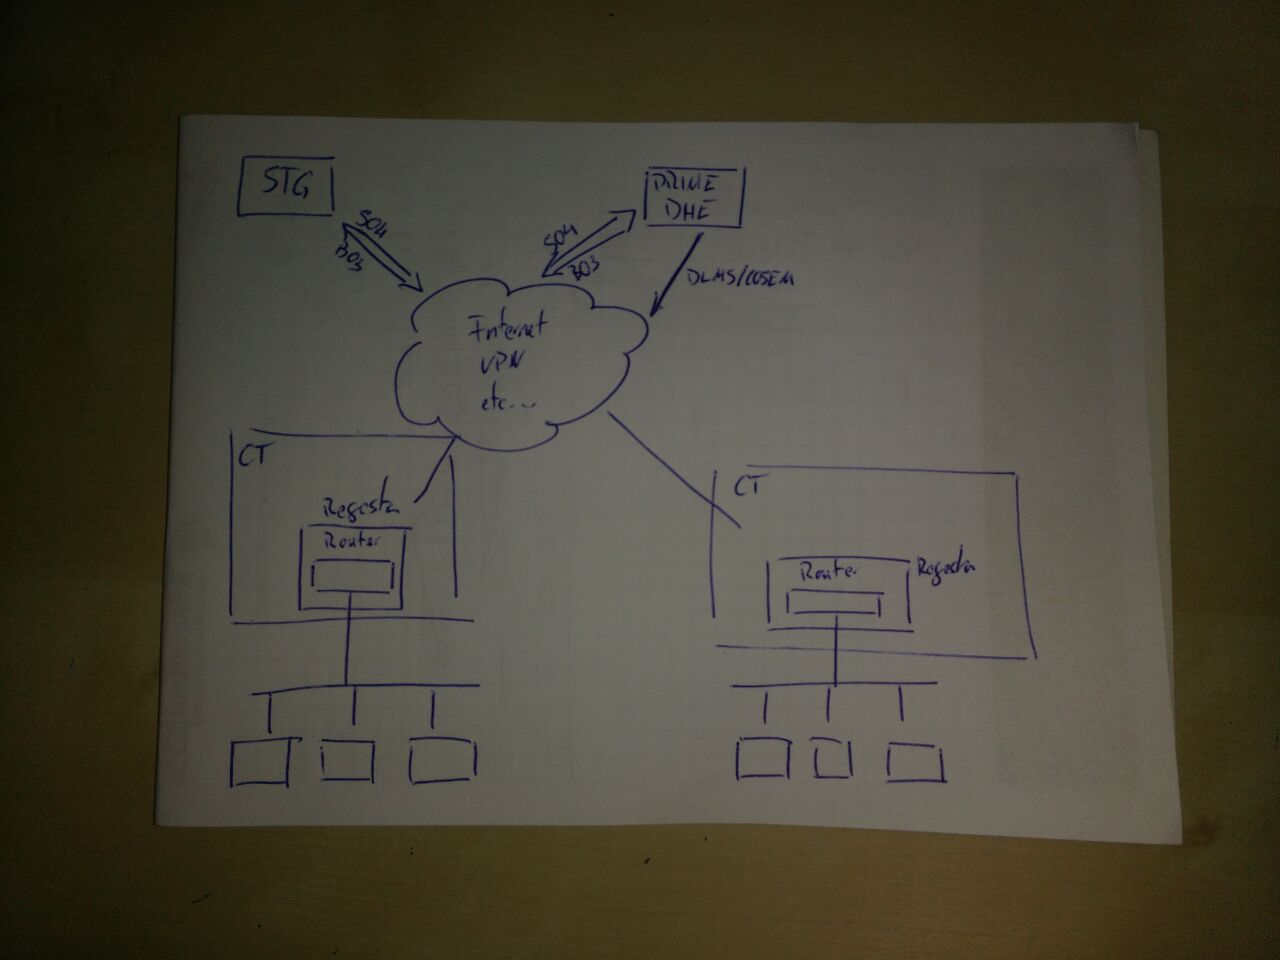
\includegraphics[width=\textwidth]{Img/boceto_red_primedhe.jpg}
	\caption{Topología de red PRIME DHE}
	\label{fig:EstructuraPrimeDHE}
\end{figure}

Por ello, la operativa tradicional bien se puede realizar por medio de un STG o bien por medio de la interfaz de la aplicación <<PRIME DHE>>. Según la topología mostrada, el sistema es perfectamente capaz de trabajar tanto con uno o con otro, o incluso pudiendo coexistir los dos a la vez. Esto propicia una adaptabilidad perfecta ante cualquier circunstancia o escenario posible.

La idea principal es la de abstraer toda complejidad posible, abarantando elementos físicos y, por ende, costes; sin que ello conlleve una disminución de características.

 Además, tal y como se puede ver en la imagen, <<PRIME DHE>> permite trabajar con más de un centro de transformación, permitiendo una modularidad e independencia de operaciones que antes no se conseguía. 
 
 \section{Arquitectura}
 
 <<PRIME DHE>> está diseñado siguiendo una arquitectura <<Cliente-Servidor>> multicapa. En líneas generales consiste en un software, al que llamaremos cliente, que realiza peticiones de datos u operaciones a otro software, al que llamaremos servidor. El servidor a su vez puede actuar como cliente de otro software servidor, etc.; repitiéndose el esquema por cada capa que compone el sistema. 
 
En este marco de funcionamiento la capacidad de proceso se reparte entre las distintas capas de clientes-servidores, con lo que se centraliza la gestión de la información y se fomenta la separación de responsabilidades; lo que facilita y clarifica el diseño del sistema.
 
 En resumen, esta arquitectura es la que mejor se adapta al escenario en el que nos movemos, ya que nos proporciona las siguientes ventajas:
 \begin{itemize}
 	\item Centralización del control
 	\item Alta escalabilidad
 	\item Fácil mantenimiento y ampliación
 	\item Mayor robustez y tolerancia a fallos
 	\item Mayor flexibilidad
 \end{itemize}






